\documentclass[tikz]{standalone}
\usepackage{etoolbox}
\usetikzlibrary{calc}

\begin{document}

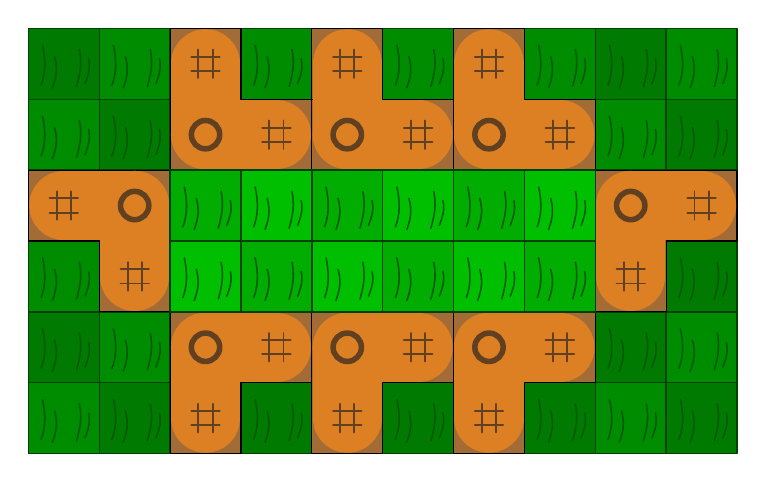
\begin{tikzpicture}[
    x=9mm,
    y=9mm,
    line cap=round,
    line join=round
]

\tikzset{
    grass border/.style={draw=green!35!black, line width=1.1pt},
    grass line/.style={draw=green!35!black, line width=0.55pt},
    wood outline/.style={draw=brown!85!black, line width=0.9pt},
    wood dark/.style={draw=brown!50!black, line width=0.7pt},
}

% ============================================================
% ONE GRASS TILE
% ============================================================
% Usage:
%   \GrassCell{x}{y}{shade}

\newcommand{\GrassCell}[3]{%
    \begin{scope}[shift={(#1,#2)}]
        \pgfmathtruncatemacro{\checker}{mod(#1+#2,2)}

        % #3 is brightness:
        %   positive = lighter
        %   negative = darker
        % Recommended range: -40 to 40
        \pgfmathtruncatemacro{\lightA}{min(100,max(0,55 + #3))}
        \pgfmathtruncatemacro{\lightB}{min(100,max(0,48 + #3))}

        % main tile
        \ifnum\checker=0
            \filldraw[
                fill=green!\lightA!black,
                draw=green!25!black,
                line width=0.5pt
            ] (0,0) rectangle (1,1);
        \else
            \filldraw[
                fill=green!\lightB!black,
                draw=green!25!black,
                line width=0.5pt
            ] (0,0) rectangle (1,1);
        \fi

        % cartoony grass blades
        \draw[grass line]
            (0.18,0.20) .. controls (0.24,0.36) and (0.25,0.54) .. (0.20,0.76);
        \draw[grass line]
            (0.34,0.16) .. controls (0.39,0.30) and (0.42,0.42) .. (0.37,0.60);
        \draw[grass line]
            (0.68,0.18) .. controls (0.73,0.36) and (0.76,0.50) .. (0.72,0.70);
        \draw[grass line]
            (0.80,0.22) .. controls (0.84,0.33) and (0.88,0.43) .. (0.85,0.57);
    \end{scope}
}

% ============================================================
% GRASS FIELD WITH GRID
% Usage: \GrassField{width}{height}
% ============================================================

\newcommand{\GrassField}[2]{%
    \pgfmathtruncatemacro{\xmax}{#1-1}
    \pgfmathtruncatemacro{\ymax}{#2-1}

    % tiles
    \foreach \x in {0,...,\xmax} {
        \foreach \y in {0,...,\ymax} {
            \GrassCell{\x}{\y}{0}
        }
    }
}

% ============================================================
% CORNER FENCE PIECES
% Usage: \CornerFence{x}{y}{NE/NW/SE/SW}
% Each occupies one full cell.
% ============================================================

\newcommand{\BaseCornerFence}[1][wood dark]{%
    \filldraw[
        fill=brown!85!black,
    ] (-1,-1) rectangle (0,1);
    \filldraw[
        fill=brown!85!black,
    ] (-1,-1) rectangle (1,0);

    \draw[orange!45!brown, line width=25pt]
        (-0.5,-0.5) -- (-0.5,0.5);
    \draw[orange!45!brown, line width=25pt]
        (-0.5,-0.5) -- (0.5,-0.5);

    \draw[wood dark] (-0.7,0.6) -- (-0.3,0.6);
    \draw[wood dark] (-0.7,0.4) -- (-0.3,0.4);
    \draw[wood dark] (-0.6,0.3) -- (-0.6,0.7);
    \draw[wood dark] (-0.4,0.3) -- (-0.4,0.7);

    \draw[#1, line width=2pt] (-0.5,-0.5) circle (0.2);

    \draw[wood dark] (0.6,-0.7) -- (0.6,-0.3);
    \draw[wood dark] (0.4,-0.7) -- (0.4,-0.3);
    \draw[wood dark] (0.3,-0.6) -- (0.7,-0.6);
    \draw[wood dark] (0.3,-0.4) -- (0.7,-0.4);
}

\newcommand{\CornerFence}[4][wood dark]{%
    \begin{scope}[shift={(#2,#3)}]
        \ifstrequal{#4}{NE}{%
            \BaseCornerFence[#1]
        }{}%

        \ifstrequal{#4}{NW}{%
            \begin{scope}[rotate=90]
                \BaseCornerFence[#1]
            \end{scope}
        }{}%

        \ifstrequal{#4}{SW}{%
            \begin{scope}[rotate=180]
                \BaseCornerFence[#1]
            \end{scope}
        }{}%

        \ifstrequal{#4}{SE}{%
            \begin{scope}[rotate=270]
                \BaseCornerFence[#1]
            \end{scope}
        }{}%
    \end{scope}
}

% Mark a rectangular area as invalid
% Usage: \InvalidMark{width}{height}
\newcommand{\InvalidMark}[2]{%
    \begin{scope}
        % optional translucent red overlay
        \fill[red!70, opacity=0.18] (0,0) rectangle (#1,#2);

        % big red X
        \draw[
            red!85!black,
            line width=7pt,
            line cap=round,
            opacity=0.85
        ] (0.25,0.25) -- ({#1-0.25},{#2-0.25});

        \draw[
            red!85!black,
            line width=7pt,
            line cap=round,
            opacity=0.85
        ] (0.25,{#2-0.25}) -- ({#1-0.25},0.25);
    \end{scope}
}


\GrassField{10}{6}

\CornerFence{3}{5}{NE}
\CornerFence{5}{5}{NE}
\CornerFence{7}{5}{NE}

\CornerFence{1}{3}{SW}
\CornerFence{9}{3}{SE}

\CornerFence{3}{1}{SE}
\CornerFence{5}{1}{SE}
\CornerFence{7}{1}{SE}


\foreach \i in {2,...,7} {
    \foreach \j in {2,...,3} {
        \GrassCell{\i}{\j}{20}
    }
}

\end{tikzpicture}

\end{document}
